\documentclass[12pt,twoside]{article}


% La extensión total de la memoria deberá ser de un máximo de 50 páginas (excluidos resumen, índice y posibles anexos).

% Según las recomendaciones de estilo, el formato de la memoria se ajustará a lo siguiente:
% ? Formato del papel: DIN A4.
% ? Impresión a dos caras.
% ? Márgenes: superior e inferior, 2.5 cm. Márgenes laterales: páginas impares, izquierdo 4 cm y derecho 2 cm; páginas % pares, izquierdo 2 cm y derecho 4 cm.
% ? Tipo de letra: Times New Roman de 12 puntos.
% ? Interlineado: 1.5 líneas.
% ? Alineación: justificación completa.
% ? Sangrado de párrafo: 0.5 cm la primera línea de cada párrafo. No se
%pondrá espacio entre párrafos.
% ? Las páginas deberán ir numeradas en números arábigos.

% Teniendo en cuenta las indicaciones previas, definimos el estilo en LaTeX:

% Indicaciones para el idioma:
\usepackage[T1]{fontenc}
\usepackage[utf8]{inputenc}
\usepackage[spanish]{babel}

% Adaptación de itemize y enumerate a los usos tipograficos españoles:
\let\layoutspanish\relax
\addto\captionsspanish{\def\tablename{Tabla}} % para que escriba "Tabla" en lugar de "Cuadro"
\unaccentedoperators  % para que no acentúe los operadores

% Área de impresión de una página:
\usepackage[a4paper]{geometry}
  \geometry{hmargin={2.5cm,2.5cm},height=22cm}

% Formato de algunas distancias:
\renewcommand{\baselinestretch}{1.2}    % separación entre líneas de un mismo párrafo
\setlength{\partopsep}{0pt}
\setlength{\itemsep}{0pt}
\setlength{\topsep}{0pt}
\setlength{\parsep}{0pt}
\setlength{\parskip}{0.25\baselineskip}   % separación entre párrafos

\renewcommand{\textfraction}{0.1}   % mínima fracción de la página para el texto
\renewcommand{\topfraction}{1}      % máxima fracción de la página para objetos flotantes en la parte superior
\renewcommand{\bottomfraction}{1}
\renewcommand{\floatpagefraction}{1}

\setcounter{totalnumber}{5}
\setcounter{topnumber}{3}
\setcounter{bottomnumber}{2}

% Adaptación de las "caption" de los entorns "figure" y "table":
\usepackage{caption}
\setcaptionwidth{\textwidth}
\addtolength{\captionwidth}{-2\parindent}
\captionsetup{margin=\leftmargini,%
  width=\captionwidth,%
  labelfont={up,bf},%
  font={small,sl},%
  %indention={\captionindent
}

% Indentación del primer párrafo de una sección:
\usepackage{indentfirst}

% Definición del color grisclaro en la salida PDF:
\usepackage[pdftex]{color}

% Gráficos:
\usepackage[pdftex]{graphicx}

% Paquetes recomendados para la inclusión de fórmulas matemáticas:
\usepackage{amsmath}
\allowdisplaybreaks  % para que pueda partir fórmulas que ocupan más de una línea, necesita el paquete anterior
\usepackage{amssymb} % para cargar algunos símbolos como \blacksquare y \square
\usepackage{amsfonts} % para cargar algunas fuentes en estilo matemático
\usepackage{enumerate}
% Teoremas (se pueden definir todos los que se necesiten):


\newtheorem{theorem}{Teorema}[section]
\newtheorem{proposition}[theorem]{Proposición}
\newtheorem{definition}[theorem]{Definición}
\newtheorem{lemma}[theorem]{Lema}
\newtheorem{corollary}[theorem]{Corolario}
\newtheorem{example}[theorem]{Ejemplo}
\newtheorem{app}[theorem]{Aplicación}
\newtheorem{remark}[theorem]{Observación}
\newtheorem{agrad}[theorem]{Agradecimiento}
\newtheorem{algo}[theorem]{Algoritmo}
\newtheorem{axiom}[theorem]{Axioma}
\newtheorem{case}[theorem]{Caso}
\newtheorem{conclu}[theorem]{Conclusión}
\newtheorem{conjectura}[theorem]{Conjetura}
\newtheorem{notac}[theorem]{Notación}
\newtheorem{soluc}[theorem]{Solución}
\newtheorem{summary}[theorem]{Sumario}

\newtheorem{proof}[theorem]{Demostración.}
\renewenvironment{proof}{\textbf{\emph{Demostración.}}} {\quad \hfill $\blacksquare$ \newline} % para que aparezca un cuadrado negro al acabar la demostración


% Definición de cabeceras y pies de página:

\usepackage{fancyhdr}                     % para definir distintos tipos de cabeceras y pies de página

\newcommand{\RunningAuthor}{Adán Avilés Cahill}
\newcommand{\Author}[1]{\renewcommand{\RunningAuthor}{#1}}
\renewcommand{\leftmark}{\RunningAuthor}

\newcommand{\RunningTitle}{Hacking Ético}
\newcommand{\Title}[1]{\renewcommand{\RunningTitle}{#1}}
\renewcommand{\rightmark}{\RunningTitle}


\pagestyle{fancy}
\fancyhf{}
\fancyhead[LO]{\small \slshape \leftmark}    % lo que aparece en la parte izquierda de la páginas impares
\fancyhead[RE]{\small \slshape \rightmark}   % lo que aparece en la parte derecha de las páginas pares
\fancyhead[RO,LE]{\small \slshape \thepage}  % el número de página aparece en la parte exterior de la cabecera

\renewcommand{\headrulewidth}{0.6pt}         % grueso de la línea horizontal por debajo de la cabecera de la página
\renewcommand{\footrulewidth}{0pt}           % grueso de la línea horizontal por encima del pie de página
                                             % en este caso está vacío
\setlength{\headheight}{1.5\headheight}      % aumenta la altura de la cabecera en una parte y media

\fancypagestyle{plain}{%                     % redefinición del estilo de página 'plain'
  \fancyhf{}                                 % limpia todas las cabeceras y pies de página
  \setlength{\headwidth}{\textwidth}
  \fancyfoot[C]{\small \slshape \thepage}    % excepto el centro del pie de página
  \renewcommand{\headrulewidth}{0pt}
  \renewcommand{\footrulewidth}{0pt}
  }

% % Instrucciones que se usan frecuentemente
% \newcommand{\abs}[1]{\ensuremath{|#1|}}
% \newcommand{\norm}[1]{\left\lVert#1\right\rVert} %norma
% \newcommand{\normd}[1]{\left\lVert#1\right\rVert_{2}} %norma
% \newcommand{\hil}{\mathcal{H} }
% \newcommand{\prodes}[2]{\langle #1, #2 \rangle }
% \newcommand{\suc}{\{x_n\}_{n=1}^{\infty}}
% \newcommand{\sumi}[2]{\sum_{#1}^{#2}}
% \newcommand{\luno}{L^1(\mathbb{R})}
% \newcommand{\ldos}{L^2(\mathbb{R})}
% \newcommand{\tf}[3]{\dfrac{1}{\sqrt{2 \pi}} \int_{-\infty}^{\infty} #1 e^{-iw#2}d#3}
% \newcommand{\erre}{\mathbb{R}}
% \newcommand{\intif}{ \int_{-\infty}^{\infty}}
% \newcommand{\cdos}{\mathcal{C}_{00}^{2} (\mathbb{R}) }
% \newcommand{\tfd}{\mathcal{F}}

% Datos del trabajo y autor:
\title{Práctica Hacking Ético}
\author{Adán Avilés Cahill\\*[1em]
\begin{minipage}{0.75\textwidth}
\footnotesize \itshape
\begin{center}
IMF BUSINESS SCHOOL\\
Máster en Ciberseguridad
\end{center}
\end{minipage}
}
\date{Junio 2014}

% Para incluir paginas de otro pdf (por ejemplo, la de la portada):
\usepackage{pdfpages}

\setlength{\abovedisplayskip}{5pt}
\setlength{\belowdisplayskip}{5pt}

\pagestyle{fancy}
%----------------------------------------------------------------------------------
%-                                  DOCUMENT START                                -
%----------------------------------------------------------------------------------
\begin{document}
\begin{figure}[t]
 \begin{picture}(140,50) \put(140,0){
\includegraphics[width=60mm]{./imagenes/logo-imf-alta}} \end{picture}
\end{figure}

\title{Análisis Forense}
\author{Adan Avilés}
\date{Junio 2020}
\maketitle


% A continuación, se incluirá el índice del trabajo y, seguidamente, se desarrollará la memoria.
\newpage
\tableofcontents
\newpage

% -------------------------------------------------% -------------------------------------------------
% -------------------------------------------------% -------------------------------------------------
% -------------------------------------------------% -------------------------------------------------
\section{Presentación del problema}
La empresa Invent S.L, que dispone de sedes en Australia, Italia y España, ha sufrido un incidente de seguridad en cada una de ellas.

% -------------------------------------------------% -------------------------------------------------
\subsection{Sede de Australia}
Por una parte, en la sede de Australia, se ha detectado la fuga de información sensible de varios de sus empleados (direcciones de correo y contraseñas). El conjunto de afectados indica haber recibido una campaña de correos sospechosos con adjuntos HTML similares al portal de Office 365 durante los últimos días. Esta empresa no tiene (2FA) factor de autenticación en dos pasos, por lo que un atacante podría acceder al correo corporativo y otro tipo de aplicativos públicos en Internet alojados en Microsoft. Puesto que hay más de 10.000 empleados en la empresa, no es posible el reseteo y bloqueo de todas las cuentas por motivos de continuidad de negocio, por lo que es necesario localizar únicamente a los afectados.
% -------------------------------------------------% -------------------------------------------------

\subsection{Sede en Italia}
Por otra parte, en Italia se ha producido un acceso no autorizado a uno de sus servidores de contabilidad. Dicho acceso ha sido detectado mediante una revisión periódica por el equipo de IT. En este caso, el equipo planea contratar a un proveedor externo para que se haga cargo de este incidente
% -------------------------------------------------% -------------------------------------------------

\subsection{Sede en España}
Finalmente, en la sede de España, se ha detectado un ataque en uno de los servidores de su fábrica de textiles. Todos los archivos del servidor han sido cifrados con la extensión “.NM4”. Estos equipos estaban parcheados contra MS17-010.

\subsubsection{Evidencias Facilitadas}
Puesto que formamos parte del equipo de respuesta ante incidentes de la compañía, nuestra misión consiste en descubrir qué ha pasado en cada una de las situaciones que se plantean.

Para ello el equipo de IT nos ha facilitado las siguientes evidencias:
\begin{itemize}
    \item Australia: logs de tráfico del proxy de navegación en el intervalo de fechas en el que se produjo el incidente.
    \item Italia: ninguna puesto que se encargará un proveedor externo.
    \item España: estado de los puertos abiertos en el sistema y parte del mensaje de rescate.
\end{itemize}

% -------------------------------------------------% -------------------------------------------------
% -------------------------------------------------% -------------------------------------------------
\newpage
% -------------------------------------------------% -------------------------------------------------
% -------------------------------------------------% -------------------------------------------------
\section{Resolución:}
Resolveremos ahora las cuestiones planteadas para cada pais.
% -------------------------------------------------% -------------------------------------------------
\subsection{Australia}
\subsubsection*{¿Qué tipo de amenaza ha impactado?}
La sede australiana ha sufrido un ataque de Ingeniería Socia, que es conocido como “Phising”.\\
Los atacantes han suplantado el loggin de \textit{Outlook} mediante una web falsa, para así poder conseguir las credenciales de los empleados que caigan en el ataque, pudiendo acceder al contenido que tengan almacenado en \textit{Office 365} y su información, además de de la empresa. \\
Para conseguir esto lo único que tuvieron que hacer es enviar un correo de forma masiva a los empleados, pidiendo que abran el archivo HTML y se loggeen en él, después esos datos se enviarían a los atacantes.


% -------------------------------------------------% -------------------------------------------------
\subsubsection*{¿Qué direcciones de correo de usuario se han visto afectadas?}
Abrimos el archivo facilitado en WireShark.
\begin{figure}[h]
    \centering
    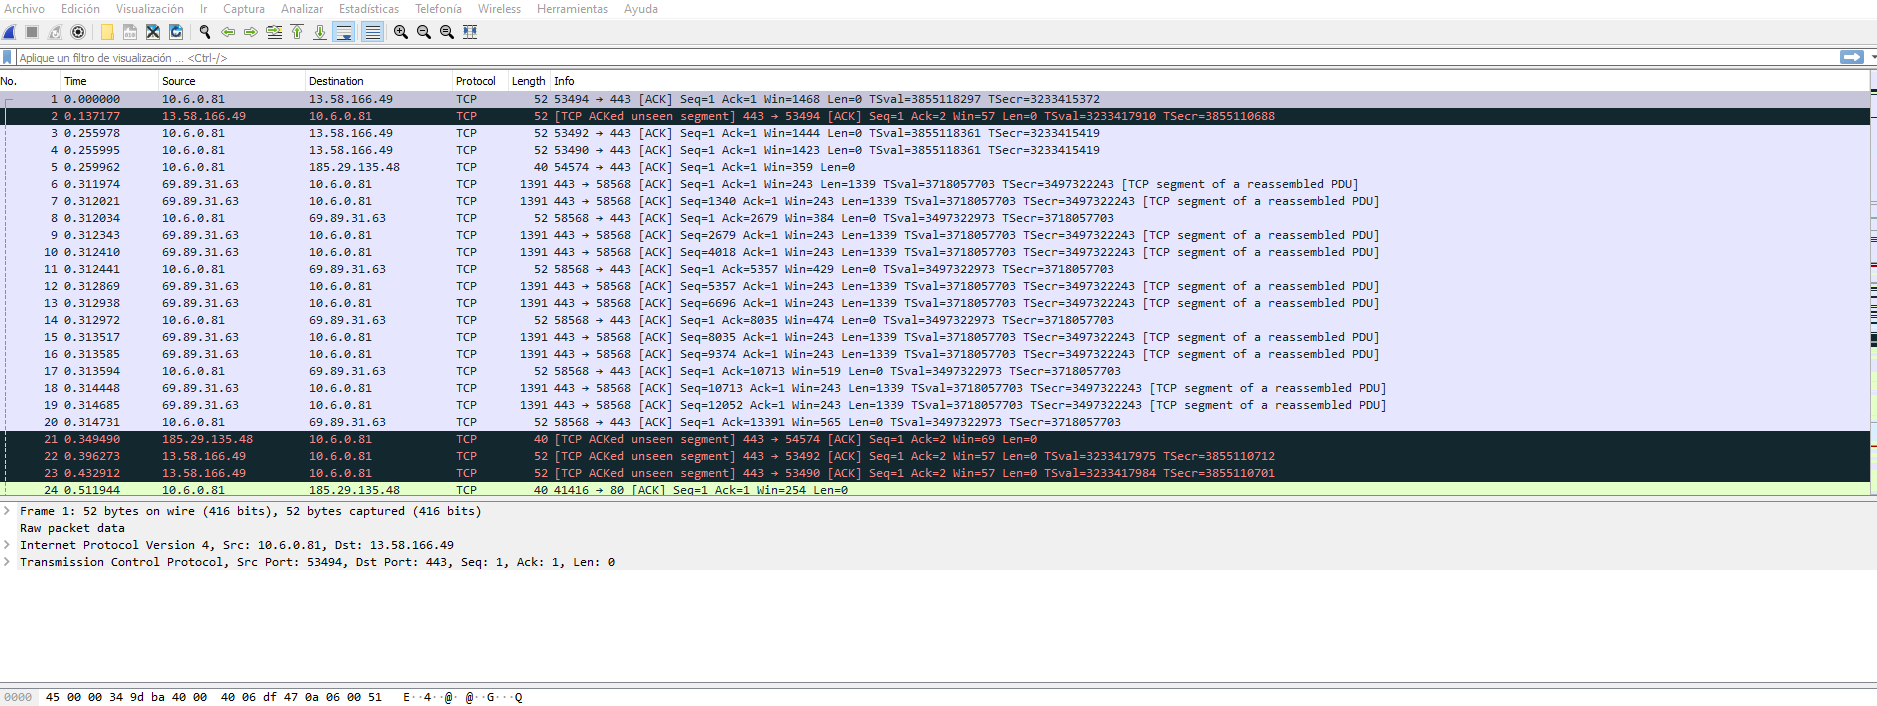
\includegraphics[scale=0.3]{./imagenes/wireshark_uno}
    \caption{Wireshark Pcap}
\end{figure}

Haciendo un filtrado en wireshark para peticiones GET (\textbf{http.request.method == "GET"}), y revisándolo, encontramos uno que en la info contiene \textit{user}, lo cual puede ser porque es un inicio de sesión.\\
Decodificamos los parámetros de la url, que aparecen en base64 obteniendo:
\begin{figure}
    \centering
    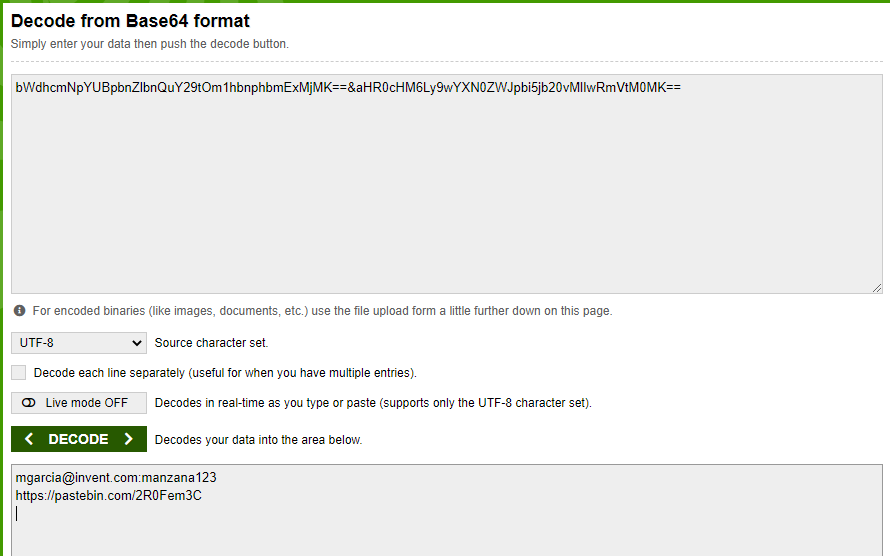
\includegraphics[scale=0.4]{./imagenes/decode}
    \caption{Parámetros decodificados}
\end{figure}
Así, si nos dirigimos al pastebien y sacamos los datos, vemos que tenemos los siguientes pares de usuario:contraseña:
\begin{itemize}
    \item mgarcia@invent.com:manzana123
    \item hifid@invent.com:123dmr
    \item hjerfs@invent.com:applepup
    \item jdarwin@invent.com:redcar\#
\end{itemize}

% -------------------------------------------------% -------------------------------------------------
\subsubsection*{Imagínese que tiene que analizar el fichero .pcap facilitado en las evidencias en un entorno linux/windows por línea de comando sin entorno gráfico. 
Realice un script para parsear el fichero .pcap, de forma que se muestre el resultado final (los correos electrónicos afectados ) por línea de comando.}

---

% -------------------------------------------------% -------------------------------------------------
% -------------------------------------------------% -------------------------------------------------
\subsection{Italia}

% -------------------------------------------------% -------------------------------------------------
\subsubsection*{Para enviar las evidencias al proveedor externo se va a realizar una captura de información y clonado del servidor comprometido. 
¿Qué parte hardware del servidor se debería clonar antes de apagar el equipo?}
La parte del hardware que deberíamos clonar sería la memoria RAM para su posterior análisis, pues al apagarlo se perderán los datos.
% -------------------------------------------------% -------------------------------------------------
\subsubsection*{¿Qué comando utilizaría para realizar el clonado del disco?}
El comando que utilizaremos será \textbf{dd}, \textit{data duplicator}. \\
La sintaxis general de este comando es 
\begin{center}
    dd if \textdblhyphen \textdollar input\textunderscore data of \textdblhyphen \textdollar output\textunderscore data
\end{center}
En nuestro caso, la dubplicación de disco a disco sería:
\begin{center}
    dd if \textdblhyphen /dev/sda1 of\textdblhyphen /dev/sdb1 bs\textdblhyphen 4096
\end{center}


% -------------------------------------------------% -------------------------------------------------
\subsubsection*{¿Qué y cómo habría que calcular después del clonado del disco para verificar la integridad del mismo?}
Tras el clonado, y habiendo tenido en cuenta que no hemos usado herramientas intrusivas que puedan alterar los datos, sino que sean conocidas o estén documentadas además de ser reproducibles, habremos de calcular el \textbf{HASH}. \\

Si el hash de ambos discos coincide, sabremos que tenemos una copia exacta del disco original. Hemos de tener en cuenta que herramientas como \textit{CAINE} calculan automáticamente el hash de la copia para poder compararlo. \\

También se puede hacer en linea de comandos con Linux. Con el comando \textbf{fdisk -l}, obtendría la lista de discos y con el comando (por ejemplo) \textbf{md5sum nombre\textunderscore de \textunderscore disco} obtendría el hash md5. 



% -------------------------------------------------% -------------------------------------------------
% -------------------------------------------------% -------------------------------------------------
\subsection{España}
% -------------------------------------------------% -------------------------------------------------
\subsubsection*{¿Qué tipo de amenaza ha impactado?}
La sede de España ha sufrido un ataque, mediante un ransonware que encripta los archivos con la extensión \textit{NM4}. Es probable que sea un ransomware que se distribuya a través de mails o de descargar programas ilícitos. \\
El objetivo de este tipo de malware es obtener beneficio económico tras solicitar de dinero para desencriptar los ficheros encriptados o "secuestrados", como podemos ver en la imagen \ref{amenaza}.

\begin{figure}
    \centering
    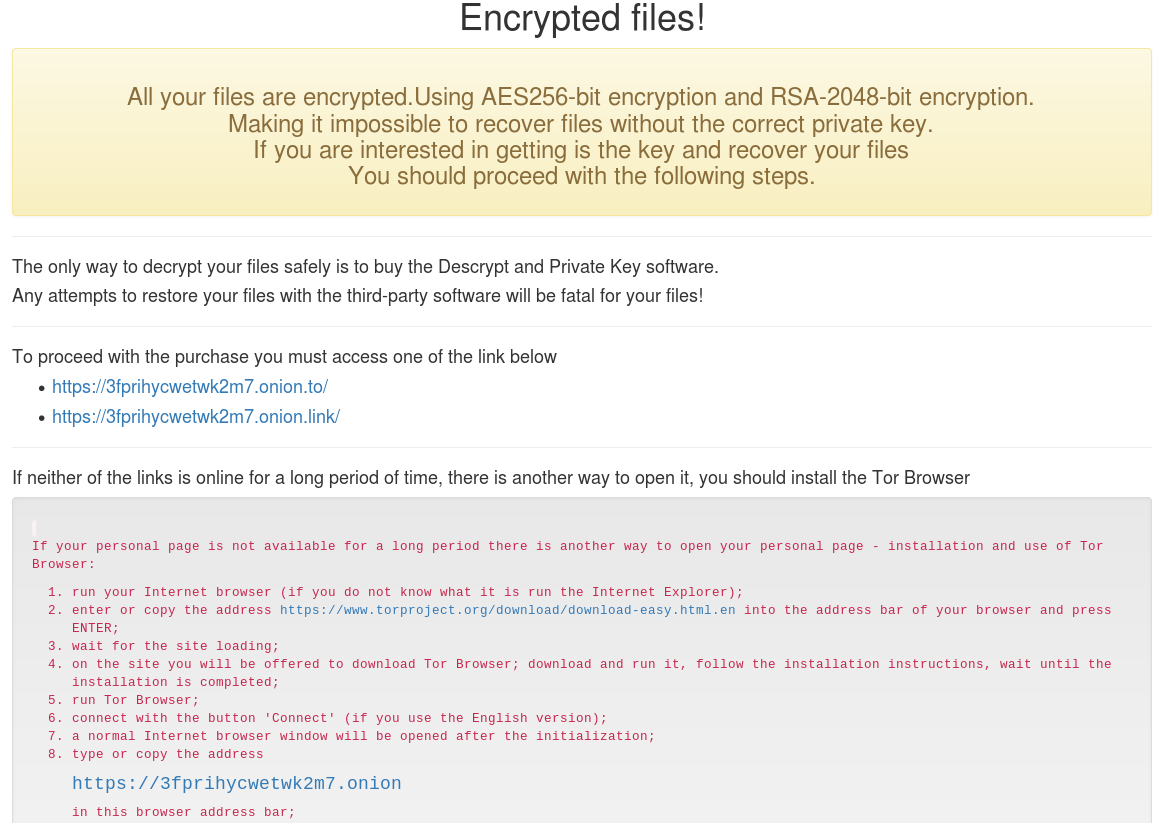
\includegraphics[scale=0.5]{./imagenes/spain_recover_files_message (1)}
    \caption{Mensaje de los atacantes}
    \label{amenaza}
\end{figure}


% -------------------------------------------------% -------------------------------------------------
\subsubsection*{¿Cómo funciona este tipo de amenaza?}
Este tipo de amenaza se basa en la infección de los ficheros por un  malware que se centra en encriptar los archivos de los usuarios con una combinación de algoritmos que no sea posible de desencriptar.\\
En particular, el virus \textit{NM4} pertenece a la familia de variantes de ransomware que emplean los algoritmos de \textit{AES} y \textit{RSA} para su  encriptación, complicando el proceso de desencriptación de los datos. \\ 
Seguidamente al haber infectado la maquina del usuario, la convierte en un bot para  replicarse por la red interna del ordenador infectado, pivotando entre los puertos abiertos. \\
Finalmente, deja en el equipo la nota o imagen que hemos visto con anterioridad, en la que están escritas las indicaciones a seguir si queremos recuperar los archivos.


% -------------------------------------------------% -------------------------------------------------
\subsubsection*{¿Cuál ha sido el vector de entrada más probable utilizado?}
Nos fijamos en las evidencias de los puertos,
\begin{figure}[h]
    \centering
    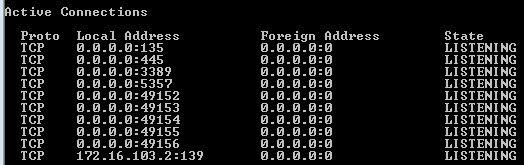
\includegraphics[scale=0.7]{./imagenes/spain (1)}
    \caption{Puertos}
\end{figure}
Sabemos que a  través del puerto SMB, como hacía \textit{EternalBlue} no es probable al estar los equipos parcheados con MS17-010, como se nos indica, así que a través de los puertos 139 o 445 no es posible haber accedido. \\ 
Un posible vector de estrada es a través del puerto 5357, pues este permite acceder usando el protocolo \textbf{Remote Desktop Protocol} (RDP) sumado a fuerza bruta de contraseñas.

% -------------------------------------------------% -------------------------------------------------
\subsubsection*{Indique 3-5 medidas imprescindibles que hubiesen evitado el ataque.}
\begin{itemize}
    \item Tener en cuenta qué puertos dejamos abiertos y sus posibles vulnerabilidades.
    \item Hacer que los empleados tengan el mínimo acceso posible a otras máquinas, para así evitar que el ransomware pivote. Para esto podemos tener la red compartimentada, no una única red con todos los equipos en ella.
    \item Tener una copia de seguridad (a ser posible diaria) de todos los archivos, para en caso de que algo así ocurra, tener siempre los archivos disponibles y solo tener que preocuparnos de recuperar los ordenadores infectados.
    \item Deshabilitar, como norma general, el Remote Desktop a no ser que sea extrictamente necesario.
    \item Filtrar los archivos ejecutables que se descargan o envían por correo.
    \item Tener instalado un antimalware actualizado.
\end{itemize}

% -------------------------------------------------% -------------------------------------------------
% -------------------------------------------------% -------------------------------------------------
% -------------------------------------------------% -------------------------------------------------







\end{document} 
